% =====================================================================
%  ZTAS-DTh journal manuscript (IEEEtran, journal mode)
%  Target: IEEE Transactions on Industrial Informatics (see cover notes)
%  Build:  pdflatex main && bibtex main && pdflatex main && pdflatex main
% =====================================================================
\documentclass[journal]{IEEEtran}
\usepackage[T1]{fontenc}
\usepackage{amsmath,amssymb,amsthm}
\usepackage{graphicx}
\usepackage{booktabs,multirow,array}
\usepackage[table]{xcolor}
\usepackage{algorithm}
\usepackage{algpseudocode}
\usepackage{tikz}
\usetikzlibrary{positioning,arrows.meta,fit,backgrounds,calc}
\usepackage[hidelinks]{hyperref}
\usepackage{cite}
\usepackage{url}

\newtheorem{definition}{Definition}
\newtheorem{proposition}{Proposition}
\newcommand{\ztas}{ZTAS-DTh}
\renewcommand{\algorithmicrequire}{\textbf{Input:}}
\renewcommand{\algorithmicensure}{\textbf{Output:}}

\begin{document}

\title{ZTAS-DTh: A Lifecycle-Spanning, Context-Adaptive Zero-Trust Security Architecture for the Digital Thread in Industrial Digital Twin Ecosystems}

\author{Muhammad~Tahir,
        Imran~Rashid,
        and~Attiq~Ahmed% <-- confirm author list, order and affiliations before submission
\thanks{The authors are with the Department of Information Security, Military College of Signals, National University of Sciences and Technology (NUST), Islamabad, Pakistan. Corresponding author: Imran Rashid (e-mail: [to be added]).}%
\thanks{This article is derived from the first author's M.S. thesis, ``Security Framework of Digital Thread in Realm of Digital Twin After 4th Industrial Revolution,'' NUST, 2026.}}

\markboth{IEEE Transactions on Industrial Informatics (submitted manuscript)}%
{Tahir \MakeLowercase{\textit{et al.}}: ZTAS-DTh: Zero-Trust Security for the Digital Thread}

\maketitle

\begin{abstract}
The digital thread (DTh) links design, manufacturing, operation and service data into one bidirectional flow that keeps industrial digital twins synchronized with their physical assets. This continuity also lets a compromise in one lifecycle phase propagate to others: a manipulated design file can corrupt machine instructions, and falsified sensor data can mislead the twin that schedules maintenance. Industrial security models protect individual zones or phases, and zero-trust architectures (ZTA) were designed for enterprise IT; neither accounts for lifecycle data lineage, twin identities or decades-long asset lifetimes. This paper presents \ztas{}, a zero-trust architecture designed around the DTh. It combines a unified identity model for humans, devices, twins and services; a five-dimensional context-aware risk engine with tiered responses and evidence accumulation; data-flow-scoped dynamic micro-segmentation; and Merkle-batched provenance signed with post-quantum signatures and verified at every phase boundary. We formalize the architecture, map it to a STRIDE threat model, and evaluate it with a reproducible Monte-Carlo propagation study on synthetic DTh graphs and with measured cryptographic costs. Under the stated assumptions, \ztas{} reduced the fraction of compromised DTh entities from 0.77--0.99 under perimeter, zone-based and static zero-trust baselines to 0.10 for a stealthy attacker, and the probability of reaching the operations phase from at least 0.70 to below 0.01. Ablation identifies phase-boundary provenance verification as the dominant mechanism. Merkle batching cut per-record ML-DSA-65 signing cost from 8.8~ms to 9.3~$\mu$s. Testbed validation remains future work.
\end{abstract}

\begin{IEEEkeywords}
Digital thread, digital twin, zero-trust architecture, Industry 4.0, cyber-physical systems, data provenance, post-quantum cryptography, micro-segmentation, threat modeling.
\end{IEEEkeywords}

% =====================================================================
\section{Introduction}
\label{sec:intro}
% =====================================================================
\IEEEPARstart{D}{igital} twins (DTs) are virtual representations of physical assets or processes that are kept synchronized with their counterparts through bidirectional data exchange and are used for monitoring, simulation and decision support~\cite{grieves2017dt,kritzinger2018dt,tao2019dt}. A twin, however, is only as current and as trustworthy as the data that reaches it. In manufacturing, that data is carried by the \emph{digital thread} (DTh): the communication and data framework that links authoritative information across the product lifecycle, from requirements and computer-aided design (CAD) through process planning, production, inspection, operation and service~\cite{helu2017dth,singh2018dth,zhang2024dth}. The twin is the destination of this data; the thread is the pathway, and it carries feedback in the opposite direction, from operational evidence back to design.

This continuity changes the security problem in three ways. First, the DTh removes the separation between phases that once limited the blast radius of an intrusion. A malicious CAD file, a poisoned simulation parameter or a tampered calibration record created in one phase is consumed, transformed and trusted in the next; propagation along data, interfaces, models and supply-chain links is a recognized property of DT ecosystems~\cite{alcaraz2022dt,mun2025survey}. Second, most of the principals on the thread are not humans. Sensors, programmable logic controllers (PLCs), analytics services and the twins themselves request and produce data, and conventional identity and access management (IAM) was not built to authenticate or reason about them~\cite{wang2023iodt}. Third, DTh records must stay verifiable for the life of the asset, which in aerospace or energy can exceed the expected lifetime of today's public-key algorithms. Attacks on industrial control systems have already shown that manipulated digital inputs can cause physical damage while operators' displays appear normal~\cite{langner2011stuxnet,cardenas2008ctrl}.

Current defenses address parts of this problem. Zone-and-conduit segmentation in IEC~62443~\cite{iec62443} and the guidance in NIST SP~800-82~\cite{stouffer2023ics} protect operational technology (OT) networks, but zones are drawn around network topology rather than lifecycle data flows. Zero-trust architecture (ZTA), as defined in NIST SP~800-207~\cite{rose2020zta}, removes implicit trust based on network location and evaluates each request, and it has been proposed for smart manufacturing~\cite{paul2023zt} and, recently, prototyped for accessing machines through their DTs~\cite{fogli2025zta}. Blockchain-based provenance has been proposed for DT data~\cite{suhail2022bdt} and for DTh traceability~\cite{krima2019dth,kuo2026multiplex}. These lines of work remain largely separate. We found no architecture that applies zero-trust enforcement to the thread \emph{as a lifecycle-spanning flow}, treats the twin as a first-class identity, verifies data lineage at phase boundaries, and quantifies how much each mechanism contributes to containing cross-phase propagation.

This paper addresses that gap. It is derived from the first author's M.S. thesis, which surveyed the DTh threat landscape and proposed the Zero Trust Adaptive Security architecture for the Digital Thread (\ztas{}). Here we formalize that architecture, correct and narrow its claims, and add a quantitative evaluation that the thesis did not contain. The contributions are as follows.
\begin{enumerate}
\item A \emph{DTh-specific threat model} that maps STRIDE threat classes to DTh components and to the cross-phase propagation channels through which a local compromise becomes a lifecycle-wide one (Section~\ref{sec:threat}).
\item The \emph{\ztas{} architecture}: five layers with a unified identity model covering twins, a five-dimensional context-aware risk engine with mode-dependent weights and evidence accumulation, data-flow-scoped dynamic micro-segmentation, and phase-boundary provenance verification over hash-chained, Merkle-batched, post-quantum-signed records (Section~\ref{sec:arch}).
\item A \emph{reproducible simulation study} of attack propagation on synthetic four-phase DTh graphs that compares \ztas{} with perimeter, zone-based and static zero-trust baselines, with ablation and sensitivity analyses that identify which mechanisms matter and under which assumptions (Sections~\ref{sec:setup}--\ref{sec:results}).
\item \emph{Measured costs} of the cryptographic primitives that \ztas{} relies on, including FIPS~203/204/205 algorithms, and a Merkle batching design that makes post-quantum signing of high-rate DTh records feasible (Section~\ref{sec:results}).
\end{enumerate}

The remainder of the paper is organized as follows. Section~\ref{sec:related} reviews related work. Section~\ref{sec:threat} defines the system and threat models. Section~\ref{sec:arch} presents \ztas{}. Section~\ref{sec:setup} describes the evaluation methodology, Section~\ref{sec:results} reports results, Section~\ref{sec:discussion} discusses implications and threats to validity, and Section~\ref{sec:conclusion} concludes.

% =====================================================================
\section{Background and Related Work}
\label{sec:related}
% =====================================================================
\subsection{Digital Twins and the Digital Thread}
Kritzinger \emph{et al.}~\cite{kritzinger2018dt} distinguish digital models, digital shadows and digital twins by whether data flows between the physical and virtual objects automatically and in one or both directions. Tao \emph{et al.}~\cite{tao2019dt} review industrial DT applications, and ISO~23247~\cite{iso23247} gives a reference framework for DTs in manufacturing. The DTh concept emerged in aerospace and defense programs and was given a manufacturing reference architecture by Helu \emph{et al.}~\cite{helu2017dth}; Singh and Willcox~\cite{singh2018dth} formalized its use for design decisions, and Zhang \emph{et al.}~\cite{zhang2024dth} review 94 DTh articles and clarify its relation to DTs, authoritative sources of truth and data linkage. Mabkhot \emph{et al.}~\cite{mabkhot2025mdp} identify security and intellectual-property risk as a reason DTh implementations remain impractical. These works define what the thread is; they treat security as a requirement rather than design it.

\subsection{Security of Digital Twin Ecosystems}
Alcaraz and Lopez~\cite{alcaraz2022dt} survey DT security threats layer by layer, and Wang \emph{et al.}~\cite{wang2023iodt} and Mun \emph{et al.}~\cite{mun2025survey} extend the taxonomy to the internet of DTs and to security requirements. Holmes \emph{et al.}~\cite{holmes2021dt} discuss the dual role of DTs as security tools and attack targets. A separate line of work uses the twin as a security instrument: Eckhart and Ekelhart run security analyses in DT-based virtual environments~\cite{eckhart2018sec,eckhart2019sota}, Dietz \emph{et al.} integrate DT security simulations into the security operations center and threat intelligence~\cite{dietz2020soc,dietz2022cti}, and It\"apelto \emph{et al.}~\cite{itapelto2025lifecycle} review DT use for lifecycle security of critical infrastructure. \ztas{} reuses this idea for pre-deployment policy testing (Section~\ref{sec:arch-intel}) but does not claim it as new.

\subsection{Zero Trust in Industrial Settings}
NIST SP~800-207~\cite{rose2020zta} defines ZTA in terms of a policy engine, policy administrator and policy enforcement points (PEPs), with access decided per session from identity, device state and other attributes. Syed \emph{et al.}~\cite{syed2022zta} survey ZTA mechanisms, and Shah \emph{et al.}~\cite{shah2021lcda} propose lightweight continuous device-to-device authentication. Paul and Rao~\cite{paul2023zt} propose a zero-trust design for smart manufacturing with micro-segmentation and device discovery. Fogli \emph{et al.}~\cite{fogli2025zta} propose design guidelines for ZTA-aware Industry~4.0 applications that access machines selectively through their DTs, and test a prototype in an industrial environment and a virtualized testbed. These works apply ZTA to access \emph{within} an operational phase. None of them treats lifecycle data lineage, cross-phase propagation or long-term verifiability.

\subsection{Provenance and Blockchain for DTs and the DTh}
Krima \emph{et al.}~\cite{krima2019dth} propose a blockchain reference model for product-data traceability along the DTh, and Hedberg \emph{et al.}~\cite{hedberg2020trace} give recommendations for the traceability and trustworthiness of manufacturing data. Joannou \emph{et al.}~\cite{joannou2020perm} show permissioned-blockchain patterns for provenance across a systems-engineering lifecycle. Suhail \emph{et al.}~\cite{suhail2022bdt} and Suleiman \emph{et al.}~\cite{suleiman2025bdt} survey blockchain-based DTs, and Kuruppuarachchi \emph{et al.}~\cite{kuruppuarachchi2022comp} address trust in composite DTs. Kuo and Yang~\cite{kuo2026multiplex} recently proposed a multiplex blockchain for DTh traceability that trades off confirmation latency and replication. These works make records tamper-evident but do not couple provenance verification to access decisions, nor do they address post-quantum signing cost.

\subsection{Positioning}
Table~\ref{tab:related} summarizes how representative works cover the capabilities that the DTh requires. The entries reflect what each work's stated scope addresses, not a judgment of its quality. \ztas{} is, to our knowledge, the first design that combines these capabilities around the thread. Unlike Fogli \emph{et al.}~\cite{fogli2025zta}, however, we do not yet report a deployed prototype; our evidence is analytical, simulated and micro-benchmarked.

\begin{table*}[!t]
\centering
\caption{Coverage of DTh security requirements by representative related work ($\bullet$ addressed; $\circ$ partially or conceptually; -- not addressed)}
\label{tab:related}
\footnotesize
\setlength{\tabcolsep}{4pt}
\begin{tabular}{@{}l l c c c c c c c@{}}
\toprule
Work & Type & Lifecycle & Twin as & Context-adaptive & Flow-scoped & Cross-phase & Post-quantum & Quantitative \\
 & & scope & identity & policy & segmentation & provenance & readiness & evaluation \\
\midrule
Alcaraz \& Lopez~\cite{alcaraz2022dt} & Survey & $\circ$ & $\circ$ & -- & -- & $\circ$ & -- & -- \\
Mun \emph{et al.}~\cite{mun2025survey} & Survey & $\circ$ & $\circ$ & -- & -- & -- & -- & -- \\
Paul \& Rao~\cite{paul2023zt} & ZT design & -- & -- & $\circ$ & $\circ$ & -- & -- & -- \\
Fogli \emph{et al.}~\cite{fogli2025zta} & ZTA + DT prototype & -- & $\circ$ & $\bullet$ & $\circ$ & -- & -- & $\bullet$ \\
Krima \emph{et al.}~\cite{krima2019dth} & Ref.\ model & $\bullet$ & -- & -- & -- & $\bullet$ & -- & -- \\
Suhail \emph{et al.}~\cite{suhail2022bdt} & Survey & $\circ$ & $\circ$ & -- & -- & $\bullet$ & -- & -- \\
Kuo \& Yang~\cite{kuo2026multiplex} & Blockchain DTh & $\bullet$ & -- & -- & -- & $\bullet$ & -- & $\bullet$ \\
Dietz \emph{et al.}~\cite{dietz2020soc} & DT security sim. & -- & -- & -- & -- & -- & -- & $\circ$ \\
\midrule
\textbf{\ztas{} (this work)} & Architecture + eval. & $\bullet$ & $\bullet$ & $\bullet$ & $\bullet$ & $\bullet$ & $\bullet$ & $\circ$\textsuperscript{a} \\
\bottomrule
\multicolumn{9}{@{}l}{\textsuperscript{a}Simulation and micro-benchmarks; testbed validation is future work (Section~\ref{sec:discussion}).}
\end{tabular}
\end{table*}

% =====================================================================
\section{System and Threat Model}
\label{sec:threat}
% =====================================================================
\subsection{System Model}
\begin{definition}[Digital thread graph]
A DTh is a directed graph $G=(V,E)$ with phase labels $\phi:V\to\Phi\cup\{X\}$, where $\Phi=\{\mathsf{D},\mathsf{M},\mathsf{O},\mathsf{S}\}$ denotes the design, manufacturing, operations and service phases and $X$ denotes external parties such as suppliers. Each vertex $v$ has a principal type $\tau(v)\in\{\text{human},\text{device},\text{twin},\text{service},\text{store}\}$. Each edge $e=(u,v)\in E$ is a data flow over which $u$ sends artifacts to $v$. An edge is \emph{cross-phase} if $\phi(u)\neq\phi(v)$.
\end{definition}
The forward flows $\mathsf{D}\!\to\!\mathsf{M}\!\to\!\mathsf{O}\!\to\!\mathsf{S}$ carry designs, instructions and operational data, and the feedback flows $\mathsf{S}\!\to\!\mathsf{D}$, $\mathsf{O}\!\to\!\mathsf{D}$ and $\mathsf{M}\!\to\!\mathsf{D}$ carry field and quality evidence back to engineering. The operations phase contains the control interfaces (PLC, DCS, SCADA) through which digital decisions cause physical effects. We therefore treat \emph{reaching} $\mathsf{O}$ as the outcome of greatest consequence.

\subsection{Adversary Model}
The adversary may (a) compromise any single entity, including a supplier account, an engineering workstation, an edge device or a service, and use that entity's credentials and network position; (b) observe, replay and inject traffic on any network segment; (c) tamper with artifacts it can write, such as CAD files, configuration, calibration records or training data; and (d) behave stealthily, keeping its observable behavior close to that of the entity it controls. We assume the adversary cannot extract keys from hardware security modules (HSMs) or physically unclonable function (PUF)-backed roots of trust, cannot forge signatures under uncompromised keys (EUF-CMA security) and cannot find collisions in SHA-256. A quantum-capable adversary may record traffic and signatures now and attack them later (``harvest now, decrypt later''). Physical destruction and denial of service at the radio layer are out of scope.

\subsection{STRIDE Threats and Propagation Channels}
Following STRIDE-based modeling for cyber-physical systems~\cite{khan2017stride,shostack2014tm}, Table~\ref{tab:stride} maps each threat class to the DTh element it targets, the channel through which it propagates across phases, and the \ztas{} control that addresses it. The thesis analysis identified four propagation channels that recur across scenarios: \emph{data-mediated} (malicious or falsified artifacts consumed downstream), \emph{interface-mediated} (stolen API or service credentials used to pivot), \emph{model-mediated} (corrupted simulation or ML models whose outputs drive decisions in later phases), and \emph{supply-chain-mediated} (compromised components, firmware or supplier identities). Representative attack scenarios include falsified quality-of-service inspection data that lets defective parts pass while the twin reports nominal behavior, manipulated process parameters or calibration records that degrade quality cumulatively, counterfeit parts introduced through cloned RFID tags or forged supplier certificates, and corrupted constraint models that sabotage production scheduling.

\begin{table*}[!t]
\centering
\caption{STRIDE threats on the DTh, their cross-phase propagation channels and the \ztas{} controls that address them}
\label{tab:stride}
\footnotesize
\renewcommand{\arraystretch}{1.1}
\begin{tabular}{@{}p{2.1cm} p{4.6cm} p{3.6cm} p{6.1cm}@{}}
\toprule
STRIDE class & DTh example & Propagation channel & \ztas{} control (Section~\ref{sec:arch}) \\
\midrule
Spoofing & Cloned sensor or PLC identity; stolen API credentials; malicious service posing as a twin & Interface; supply chain & Hardware-rooted device identity (HSM/PUF), twin identities bound to model hashes, short-lived service certificates (\ref{sec:arch-id}) \\
Tampering & Falsified sensor data; altered CAD, G-code, calibration or quality records & Data & Hash-chained provenance, signatures at the source, verification at every phase boundary (\ref{sec:arch-prov}) \\
Repudiation & Unattributable design change or command & Data & Signed records bound to actor, session and purpose; append-only ledger (\ref{sec:arch-prov}) \\
Information disclosure & Exfiltration of design IP or process parameters by a supplier or insider & Interface; supply chain & Purpose-bound, time-limited segments; business-sensitivity dimension of risk (\ref{sec:arch-seg},\ref{sec:arch-risk}) \\
Denial of service & Flooding data-ingress gateways; ransomware on historians & Interface & Edge-gateway admission control; isolation tier; availability monitoring (\ref{sec:arch-risk}) \\
Elevation of privilege & Pivot from low-privilege device to control interface; poisoned model drives actuation & Model; interface & Per-request evaluation, least-privilege segments, step-up and quarantine, model-integrity checks (\ref{sec:arch-risk},\ref{sec:arch-seg}) \\
\bottomrule
\end{tabular}
\end{table*}

% =====================================================================
\section{The \ztas{} Architecture}
\label{sec:arch}
% =====================================================================
\subsection{Design Assumptions and Principles}
\ztas{} follows the zero-trust tenets of SP~800-207~\cite{rose2020zta} and adds one industrial constraint. Its assumptions are: (A1) every flow is untrusted regardless of origin or network location; (A2) privileges are granted per transaction and are revocable; (A3) verification is continuous rather than performed once per session; (A4) any entity may already be compromised, so the design must detect and contain; and (A5) security controls must not violate the timing requirements of the production process. From these assumptions follow three principles that distinguish \ztas{} from an IT ZTA deployed in a factory: \emph{context-aware continuous verification} that includes manufacturing context, \emph{segmentation by data flow rather than by subnet}, and \emph{verification of lineage at the points where data changes hands between lifecycle phases}.

\subsection{Layered Architecture}
Fig.~\ref{fig:arch} shows the five layers. The \emph{physical-world layer} contains assets, sensors and actuators, secure edge gateways that act as the first PEPs, and HSMs that hold device keys. The \emph{framework core} hosts identity management, the context-aware policy engine, the segmentation controller, the provenance service and adaptive risk monitoring. The \emph{DTh execution layer} applies phase-specific controls to design, manufacturing, operations and service. The \emph{security intelligence layer} provides threat intelligence, behavioral analytics, DT-based security simulation and the audit ledger. The \emph{management and orchestration layer} exposes dashboards, policy management, compliance mapping and incident-response playbooks. The layers exchange feedback: incidents update behavioral baselines and weights, and simulation results update policy before deployment.

\begin{figure*}[!t]
\centering
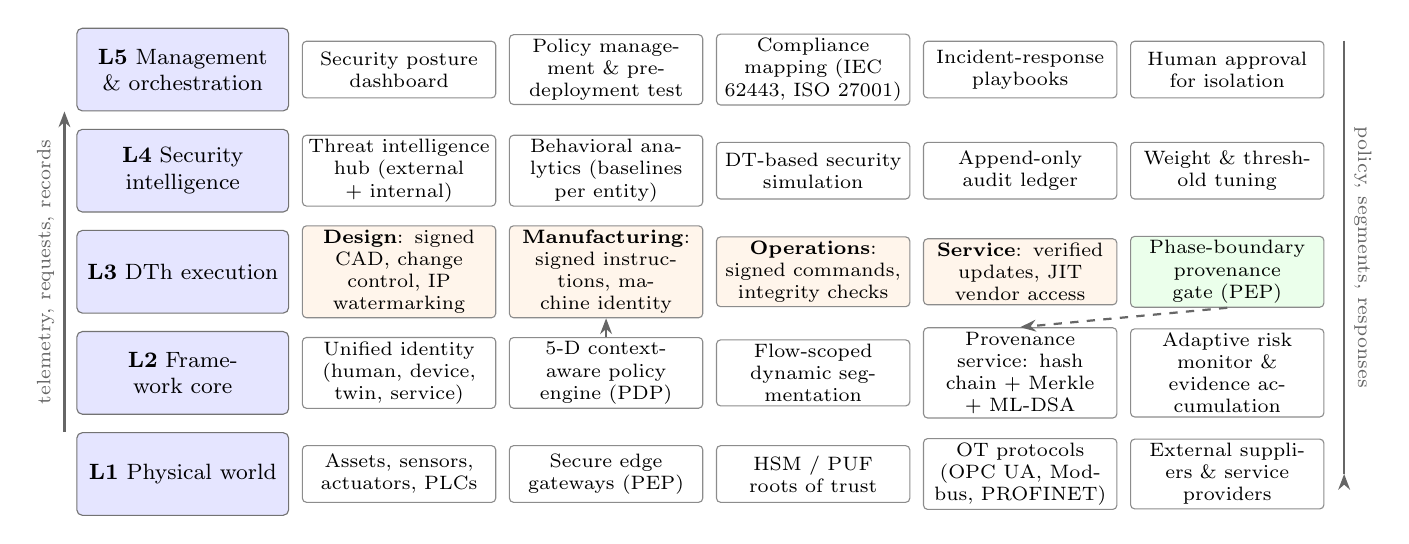
\begin{tikzpicture}[
  font=\footnotesize,
  layer/.style={draw=black!55, rounded corners=2pt, fill=#1, minimum height=1.05cm, text width=2.55cm, align=center, inner sep=2pt},
  comp/.style={draw=black!45, rounded corners=1.5pt, fill=white, minimum height=0.72cm, text width=2.35cm, align=center, inner sep=1.5pt, font=\scriptsize},
  arr/.style={-{Stealth[length=2mm]}, thick, black!60},
  node distance=0.18cm and 0.16cm]
% layer labels
\node[layer=blue!10]   (L5) {\textbf{L5} Management \& orchestration};
\node[layer=blue!10, below=0.22cm of L5] (L4) {\textbf{L4} Security intelligence};
\node[layer=blue!10, below=0.22cm of L4] (L3) {\textbf{L3} DTh execution};
\node[layer=blue!10, below=0.22cm of L3] (L2) {\textbf{L2} Framework core};
\node[layer=blue!10, below=0.22cm of L2] (L1) {\textbf{L1} Physical world};
% L5
\node[comp, right=of L5] (a1) {Security posture dashboard};
\node[comp, right=of a1] (a2) {Policy management \& pre-deployment test};
\node[comp, right=of a2] (a3) {Compliance mapping (IEC 62443, ISO 27001)};
\node[comp, right=of a3] (a4) {Incident-response playbooks};
\node[comp, right=of a4] (a5) {Human approval for isolation};
% L4
\node[comp, right=of L4] (b1) {Threat intelligence hub (external + internal)};
\node[comp, right=of b1] (b2) {Behavioral analytics (baselines per entity)};
\node[comp, right=of b2] (b3) {DT-based security simulation};
\node[comp, right=of b3] (b4) {Append-only audit ledger};
\node[comp, right=of b4] (b5) {Weight \& threshold tuning};
% L3
\node[comp, right=of L3, fill=orange!8] (c1) {\textbf{Design}: signed CAD, change control, IP watermarking};
\node[comp, right=of c1, fill=orange!8] (c2) {\textbf{Manufacturing}: signed instructions, machine identity};
\node[comp, right=of c2, fill=orange!8] (c3) {\textbf{Operations}: signed commands, integrity checks};
\node[comp, right=of c3, fill=orange!8] (c4) {\textbf{Service}: verified updates, JIT vendor access};
\node[comp, right=of c4, fill=green!8] (c5) {Phase-boundary provenance gate (PEP)};
% L2
\node[comp, right=of L2] (d1) {Unified identity (human, device, twin, service)};
\node[comp, right=of d1] (d2) {5-D context-aware policy engine (PDP)};
\node[comp, right=of d2] (d3) {Flow-scoped dynamic segmentation};
\node[comp, right=of d3] (d4) {Provenance service: hash chain + Merkle + ML-DSA};
\node[comp, right=of d4] (d5) {Adaptive risk monitor \& evidence accumulation};
% L1
\node[comp, right=of L1] (e1) {Assets, sensors, actuators, PLCs};
\node[comp, right=of e1] (e2) {Secure edge gateways (PEP)};
\node[comp, right=of e2] (e3) {HSM / PUF roots of trust};
\node[comp, right=of e3] (e4) {OT protocols (OPC UA, Modbus, PROFINET)};
\node[comp, right=of e4] (e5) {External suppliers \& service providers};
% arrows between layers (feedback loop)
\draw[arr] ([xshift=-0.15cm]L1.north west) -- ([xshift=-0.15cm]L5.south west) node[midway, left, rotate=90, anchor=south, font=\scriptsize] {telemetry, requests, records};
\draw[arr] ([xshift=0.25cm]a5.north east) |- ([xshift=0.25cm,yshift=0cm]e5.east) node[pos=0.25, right, rotate=-90, anchor=south, font=\scriptsize] {policy, segments, responses};
\draw[arr, dashed] (c5.south) -- (d4.north);
\draw[arr, dashed] (d2.north) -- (c2.south);
\end{tikzpicture}
\caption{The five-layer \ztas{} architecture. Edge gateways and phase-boundary provenance gates act as policy enforcement points (PEPs); the context-aware policy engine is the policy decision point (PDP). Telemetry and decisions form a closed loop across layers.}
\label{fig:arch}
\end{figure*}

\subsection{Unified Identity for Humans, Devices, Twins and Services}
\label{sec:arch-id}
Every principal receives an identity at creation, and the identity is revoked when the principal is decommissioned. Human users authenticate with phishing-resistant multi-factor authentication and are continuously checked against behavioral baselines. Devices hold keys generated in an HSM or derived from a PUF, so that a cloned device cannot present a valid credential. Services receive short-lived certificates and are code-signed. A \emph{digital twin} receives its own identity, bound to the hash of its model and configuration, so that a twin whose model has been altered no longer matches its identity and cannot request data under it. This addresses a gap noted in DT security surveys~\cite{alcaraz2022dt,mun2025survey}: twins are usually treated as data rather than as principals that act. Identities and long-lived signatures use NIST-standardized post-quantum algorithms: ML-KEM (FIPS~203)~\cite{fips203} for key establishment and ML-DSA (FIPS~204)~\cite{fips204} for signatures, with SLH-DSA (FIPS~205)~\cite{fips205} as a conservative alternative for root keys. During migration, hybrid classical-plus-PQ modes preserve interoperability with legacy endpoints.

\subsection{Context-Aware Risk Engine}
\label{sec:arch-risk}
A request is a tuple $q=(s,o,a,c)$ of subject, object, action and context. The policy engine computes five normalized risk components $\rho_k(q)\in[0,100]$: \emph{temporal} (deviation from shift patterns), \emph{spatial} (physical and network location), \emph{behavioral} (deviation from the subject's learned baseline), \emph{system} (device health and attestation state) and \emph{business} (data sensitivity and regulatory impact). The risk score is
\begin{equation}
r(q)=\sum_{k=1}^{5} w_k(m)\,\rho_k(q),\qquad \mathbf{w}(m)\in\Delta^4,
\label{eq:risk}
\end{equation}
where $\Delta^4$ is the probability simplex and the weight vector $\mathbf{w}(m)$ depends on the operating mode $m$ (e.g., design review, production, maintenance). In production, for example, the behavioral and system components carry more weight than the temporal one, because shift patterns are regular and device integrity directly affects the physical process. The engine maps $r(q)$ to four tiers with thresholds $\boldsymbol{\theta}=(30,70,90)$: \emph{allow} and log ($r\le30$), \emph{step-up} authentication or device re-attestation ($30<r\le70$), \emph{block} with alert and evidence preservation ($70<r\le90$), and \emph{isolate} the subject ($r>90$).

A single request rarely carries enough evidence to reach the upper tiers; Section~\ref{sec:results} shows this quantitatively. \ztas{} therefore accumulates evidence: each failed step-up increments a per-subject counter $c_s$, and the subject is quarantined when $c_s\ge\kappa$. This is the continuous adaptive trust idea of ZTA expressed as a concrete rule. Because isolation in OT can itself cause harm, isolation of safety-relevant assets is routed to a human operator through Layer~5 rather than executed automatically. Algorithm~\ref{alg:pdp} summarizes the decision procedure at a PEP.

\begin{algorithm}[!t]
\caption{Policy decision and enforcement at a \ztas{} PEP}
\label{alg:pdp}
\begin{algorithmic}[1]
\Require request $q=(s,o,a,c)$ on flow $e=(u,v)$ at time $t$; mode $m$
\Ensure decision $\in\{\textsc{Allow},\textsc{Deny},\textsc{Isolate}\}$
\If{$s$ quarantined \textbf{or} identity/attestation of $s$ invalid} \State \Return \textsc{Deny}
\EndIf
\If{no active segment $\sigma$ with $e\in F_\sigma$, $s\in\Pi_\sigma$, $t\in[t^{\mathrm{s}}_\sigma,t^{\mathrm{e}}_\sigma]$} \State \Return \textsc{Deny}
\EndIf
\If{$\phi(u)\neq\phi(v)$ \textbf{and} \Call{VerifyLineage}{artifact of $q$} fails} \State alert; \Return \textsc{Isolate}
\EndIf
\State $r\gets\sum_k w_k(m)\rho_k(q)$ \Comment{Eq.~\eqref{eq:risk}}
\If{$r>\theta_3$} \State \Return \textsc{Isolate} \Comment{operator approval for safety assets}
\ElsIf{$r>\theta_2$} \State alert, preserve evidence; \Return \textsc{Deny}
\ElsIf{$r>\theta_1$}
  \If{\Call{StepUp}{$s$} fails} \State $c_s\gets c_s+1$
     \If{$c_s\ge\kappa$} \Return \textsc{Isolate} \EndIf
     \State \Return \textsc{Deny}
  \EndIf
\EndIf
\State append signed provenance record; \Return \textsc{Allow}
\end{algorithmic}
\end{algorithm}

\subsection{Flow-Scoped Dynamic Micro-Segmentation}
\label{sec:arch-seg}
A segment is a tuple $\sigma=(F_\sigma,\Pi_\sigma,\pi_\sigma,[t^{\mathrm{s}}_\sigma,t^{\mathrm{e}}_\sigma])$: a set of flows, the principals allowed on them, a declared purpose and a validity window. An edge is reachable at time $t$ only while some segment that contains it is active. Segments are created for activities, such as a design review, a supplier data exchange, an emergency maintenance window or an audit, and are dissolved when the activity ends. Static zones, by contrast, keep every legitimate flow open permanently. Because segments are defined over DTh relationships rather than IP subnets, they apply equally to on-premises, edge and cloud components, and an expired segment closes the paths that an attacker would otherwise use for lateral movement.

\subsection{Phase-Boundary Provenance Verification}
\label{sec:arch-prov}
Every artifact that enters or is transformed on the thread produces a provenance record
\begin{multline}
\rho_i=\bigl(\mathit{id},\,\mathit{src},\,H(\mathit{data}),\,\mathit{op},\,\{H(\rho_p)\}_{p\in\mathrm{par}(i)},\\
\mathit{actor},\,\mathit{purpose},\,t_i\bigr),
\end{multline}
which names its source, content hash, transformation, parent records, acting principal, purpose and timestamp. Records produced by a node are hash-chained, $h_i=H(\rho_i\,\|\,h_{i-1})$, which makes deletion or reordering detectable~\cite{crosby2009log}. To make post-quantum signing affordable at sensor rates, records are collected into batches of size $B$; the batch's Merkle root $R_j$~\cite{merkle1987sig} is signed with ML-DSA inside the gateway HSM and anchored on a permissioned ledger shared by the manufacturer and its partners~\cite{krima2019dth,joannou2020perm}. A record is then authenticated by one signature verification plus an inclusion proof of $\lceil\log_2 B\rceil$ hashes.

The provenance gate at each cross-phase flow (Algorithm~\ref{alg:pdp}) checks the signature, the inclusion proof, and a \emph{lineage policy} that lists which transformations and actors are admissible for that artifact type, e.g., ``machine instructions must derive from a released design revision through an approved CAM post-processor.''

\begin{proposition}
Let an artifact $x$ cross a phase boundary with record $\rho$ included under root $R$, where $R$ carries a valid ML-DSA signature under the key of an uncompromised gateway. If $x$ or $\rho$ was altered after signing, the gate rejects it except with probability negligible in the security parameter.
\end{proposition}
\begin{IEEEproof}[Proof sketch]
Acceptance of an altered $x'$ requires either $H(x')=H(x)$, a SHA-256 collision, or an altered $\rho'$ whose inclusion proof verifies against $R$, again a collision, or a valid signature on a root $R'\neq R$, which is an EUF-CMA forgery. Each event has negligible probability under the stated assumptions.
\end{IEEEproof}
The proposition does \emph{not} cover data that is false when first signed, e.g., a falsified reading from a tampered sensor, or artifacts signed by an entity the adversary controls. Such data passes signature checks, and the lineage policy and behavioral analytics must catch it instead. This limit is why the simulation in Section~\ref{sec:setup} models provenance detection as a probability $p_v<1$ rather than as certainty.

\subsection{Lifecycle Controls}
Table~\ref{tab:lifecycle} lists the phase-specific controls in the DTh execution layer. The service phase closes the loop: it governs software updates, third-party maintenance and the feedback of field data into design, which are the channels through which supply-chain and model-mediated attacks re-enter the thread.

\begin{table}[!t]
\centering
\caption{Phase-specific controls in the DTh execution layer}
\label{tab:lifecycle}
\footnotesize
\begin{tabular}{@{}p{1.65cm}p{2.9cm}p{3.1cm}@{}}
\toprule
Phase & Assets protected & Controls \\
\midrule
Design & CAD models, simulation parameters, requirements & Signed revisions; change approval on ledger; forensic watermarking; PQ encryption at rest \\
Manufacturing & Process plans, G-code, machine instructions, quality records & Instructions verified against released design lineage; hardware-rooted machine identity; signed quality records \\
Operations & Sensor streams, control commands, twin state & Real-time integrity checks; signed commands with HSM keys; just-in-time remote access; anomaly detection \\
Service & Updates, maintenance records, field feedback & Signed updates with rollback protection; time- and scope-limited vendor tokens; authenticated feedback channels \\
\bottomrule
\end{tabular}
\end{table}

\subsection{Security Intelligence and DT-Based Simulation}
\label{sec:arch-intel}
The intelligence layer combines external threat feeds with internal incident data, maintains per-entity behavioral baselines for users, device communication, data volumes and process timing, and stores security events in the append-only ledger. Following prior work on DT-based security simulation~\cite{eckhart2018sec,dietz2020soc}, \ztas{} uses the twins it protects to replay attack scenarios, such as ransomware spreading along the thread, a compromised supplier credential or sensor manipulation, and to test policy changes before deployment. Our contribution here is integration with the policy loop, not the simulation technique itself.

% =====================================================================
\section{Evaluation Methodology}
\label{sec:setup}
% =====================================================================
The thesis validated \ztas{} only conceptually. To obtain quantitative evidence without an industrial testbed, we ran three reproducible experiments. Their purpose is to measure the \emph{relative} effect of the architectural mechanisms under explicit assumptions and the \emph{absolute} cost of the cryptographic primitives. They are not measurements of a deployed system. All code, parameters and raw results are provided as supplementary material.

\subsection{E1: Cross-Phase Propagation Simulation}
\emph{Graph generation.} Each synthetic DTh has 14 internal entities per phase (56 in total) with intra-phase flows drawn independently with probability 0.3, six cross-phase flows for each of the forward and feedback pairs $\mathsf{D}\!\to\!\mathsf{M}$, $\mathsf{M}\!\to\!\mathsf{O}$, $\mathsf{O}\!\to\!\mathsf{S}$, $\mathsf{S}\!\to\!\mathsf{D}$, $\mathsf{O}\!\to\!\mathsf{D}$ and $\mathsf{M}\!\to\!\mathsf{D}$, and four external suppliers with flows into $\mathsf{D}$, $\mathsf{M}$ and $\mathsf{S}$. We used ten graph instances.

\emph{Attack process.} An attack starts at a uniformly chosen supplier or design, manufacturing or service entity. At each of $T=60$ steps, every compromised and non-isolated entity attempts each outgoing flow, and succeeds with probability $p_x=0.3$ modified by the active defense. We ran 1000 Monte-Carlo runs per configuration (100 per graph) and report means with 95\% confidence intervals.

\emph{Configurations.} (i) \emph{Perimeter}: no internal control. (ii) \emph{Static zones}: one zone per phase in the spirit of IEC~62443 zones and conduits; conduit inspection halves $p_x$ on cross-phase flows and detects a crossing attempt with probability 0.2. (iii) \emph{Static ZT}: per-request authentication defeats a lateral move with probability $p_a=0.5$, and generic anomaly detection isolates a compromised node with probability 0.05 per step. (iv) \emph{\ztas{}}: per-request authentication as in (iii), plus flow segments open with probability $p_{\mathrm{act}}=0.3$ per step, the risk engine of Eq.~\eqref{eq:risk} with tiers and evidence accumulation ($\kappa=2$, step-up failure probability 0.7), and phase-boundary provenance verification that detects a tampered artifact with probability $p_v=0.9$.

\emph{Risk scores.} For legitimate requests, each component is drawn from $\mathcal{N}(15,8^2)$, clipped to $[0,100]$. For malicious requests the behavioral component is drawn from $\mathcal{N}(\mu_{\mathrm{mal}},15^2)$, and, with probability 0.5 (degraded device integrity), so is the system component. We evaluate a \emph{noisy} attacker ($\mu_{\mathrm{mal}}=55$) and a \emph{stealthy} attacker ($\mu_{\mathrm{mal}}=28$). The production-mode weights are $\mathbf{w}=(0.10,0.10,0.35,0.30,0.15)$, compared with uniform weights $w_k=0.2$.

\emph{Metrics.} The fraction of internal entities compromised at $T$; the probability that the attack reaches the operations phase; and the isolation ratio, i.e., the fraction of compromised entities isolated by $T$.

\emph{Ablation and sensitivity.} Under the stealthy profile, we remove each \ztas{} mechanism in turn, and we sweep $\mu_{\mathrm{mal}}\in[15,55]$, $p_{\mathrm{act}}\in[0.1,1]$ and $p_v\in[0,0.99]$ with 500 runs per point.

\subsection{E2: Operating Characteristic of the Risk Engine}
We drew $2\times10^4$ legitimate and $2\times10^4$ malicious requests from the distributions above and computed, for every threshold $\theta\in[0,100]$, the fraction of each escalated beyond \emph{allow}. We also recorded how the thesis thresholds $\boldsymbol{\theta}=(30,70,90)$ distribute requests across tiers.

\subsection{E3: Cryptographic Cost Measurements}
We measured, on one core of an Intel Xeon processor at 2.10~GHz (2 vCPUs, Linux, Python~3.13), the median and 95th-percentile latency of SHA-256 hash chaining of 256-byte records; signing and verification with Ed25519, ECDSA P-256 (OpenSSL via \texttt{cryptography}~50.0.1), ML-DSA-44, ML-DSA-65 and SLH-DSA-SHA2-128f (\texttt{pqcrypto}~1.0.0); X25519 versus ML-KEM-768 key establishment; Merkle batching with ML-DSA-65 for $B\in\{1,\dots,1024\}$; and evaluation of Eq.~\eqref{eq:risk} with tiering. Each signature measurement used 3000 repetitions after warm-up (100 for SLH-DSA). The PQ library uses portable implementations without platform-specific vector optimizations, so its timings are conservative.

% =====================================================================
\section{Results}
\label{sec:results}
% =====================================================================
\subsection{Containment of Cross-Phase Propagation}
Table~\ref{tab:main} and Fig.~\ref{fig:prop} report E1. Without internal controls, attacks spread to almost the whole thread (0.994 of entities) and reached operations in 99.9\% of runs. Static zones reduced spread to 0.765 and operations reach to 0.703, because conduits slow but do not stop movement along legitimate cross-phase flows. Static ZT reached a higher isolation ratio (0.900) but still let 0.847 of entities be compromised, because generic detection acted after the attack had spread. The two attacker profiles give identical results for the three baselines, which do not use the risk score.

\ztas{} reduced the compromised fraction to 0.022 for the noisy attacker and to 0.100 for the stealthy one. Operations was reached in 0 of 1000 runs for the noisy attacker and in 0.9\% of runs for the stealthy one. Compared with the best baseline on each metric, this is a 7.7-fold reduction in spread for the stealthy attacker and a reduction in operations reach from 0.703 to 0.009.

\begin{table*}[!t]
\centering
\caption{E1: Propagation outcomes after $T=60$ steps (mean $\pm$ 95\% CI over 1000 runs on 10 synthetic DTh graphs)}
\label{tab:main}
\footnotesize
\begin{tabular}{@{}lccccc@{}}
\toprule
 & \multicolumn{2}{c}{Noisy attacker ($\mu_{\mathrm{mal}}=55$)} & \multicolumn{3}{c}{Stealthy attacker ($\mu_{\mathrm{mal}}=28$)} \\
\cmidrule(lr){2-3}\cmidrule(lr){4-6}
Configuration & Fraction compromised & P(reach operations) & Fraction compromised & P(reach operations) & Isolation ratio \\
\midrule
Perimeter (flat trust) & 0.994 $\pm$ 0.002 & 0.999 $\pm$ 0.002 & 0.994 $\pm$ 0.002 & 0.999 $\pm$ 0.002 & 0.000 \\
Static zones/conduits & 0.765 $\pm$ 0.021 & 0.703 $\pm$ 0.028 & 0.765 $\pm$ 0.021 & 0.703 $\pm$ 0.028 & 0.246 \\
Static zero trust & 0.847 $\pm$ 0.019 & 0.870 $\pm$ 0.021 & 0.847 $\pm$ 0.019 & 0.870 $\pm$ 0.021 & 0.900 \\
ZTAS-DTh (proposed) & 0.022 $\pm$ 0.001 & 0.000 $\pm$ 0.000 & 0.100 $\pm$ 0.006 & 0.009 $\pm$ 0.006 & 0.773 \\
\bottomrule
\end{tabular}
\end{table*}

\begin{figure*}[!t]
\centering
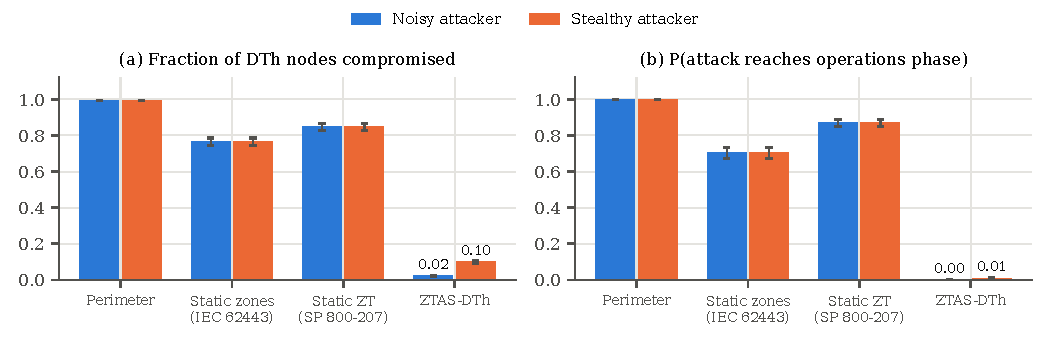
\includegraphics[width=\textwidth]{figs/fig_propagation.pdf}
\caption{E1: (a) mean fraction of DTh entities compromised and (b) probability that the attack reaches the operations phase, for four security configurations and two attacker profiles. Error bars are 95\% confidence intervals.}
\label{fig:prop}
\end{figure*}

\subsection{Which Mechanisms Matter}
Fig.~\ref{fig:abl} shows the ablation under the stealthy profile. Removing phase-boundary provenance verification increased the compromised fraction from 0.100 to 0.542 and the probability of reaching operations from 0.009 to 0.636; it is the dominant mechanism. Removing the risk engine raised spread to 0.134 and lowered the isolation ratio from 0.773 to 0.626. Replacing the production-mode weights with uniform weights had a similar effect (0.143). Removing dynamic segmentation had the smallest effect (0.119). With authentication alone, the outcome was indistinguishable from the perimeter baseline (0.991), which confirms that per-request authentication cannot contain an adversary that holds a compromised entity's credentials.

\begin{figure}[!t]
\centering
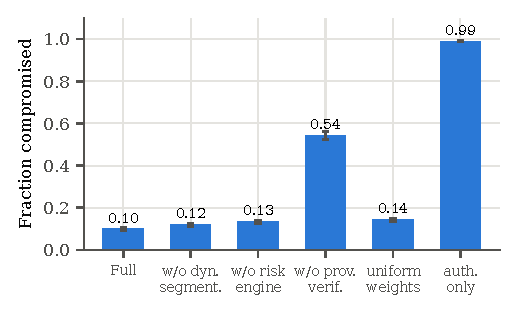
\includegraphics[width=\columnwidth]{figs/fig_ablation.pdf}
\caption{E1 ablation (stealthy attacker): fraction compromised when each \ztas{} mechanism is removed. ``Auth.\ only'' keeps per-request authentication and removes all other mechanisms.}
\label{fig:abl}
\end{figure}

The sensitivity analysis (Fig.~\ref{fig:sens}) explains this ordering. As the attacker becomes stealthier ($\mu_{\mathrm{mal}}\to15$, the legitimate mean), the risk engine's contribution vanishes and the isolation ratio falls from 0.997 to 0.604, but spread stays bounded at 0.142 because provenance checks at phase boundaries do not depend on behavioral separability. Conversely, spread and operations reach rise steeply as $p_v$ falls: at $p_v=0.5$ the attack reached operations in 8.8\% of runs, and at $p_v=0$ in 62.6\%. The segment-open probability $p_{\mathrm{act}}$ mainly delays spread. Over 60 steps, the compromised fraction varied only between 0.059 and 0.116 across $p_{\mathrm{act}}\in[0.1,1]$.

\begin{figure*}[!t]
\centering
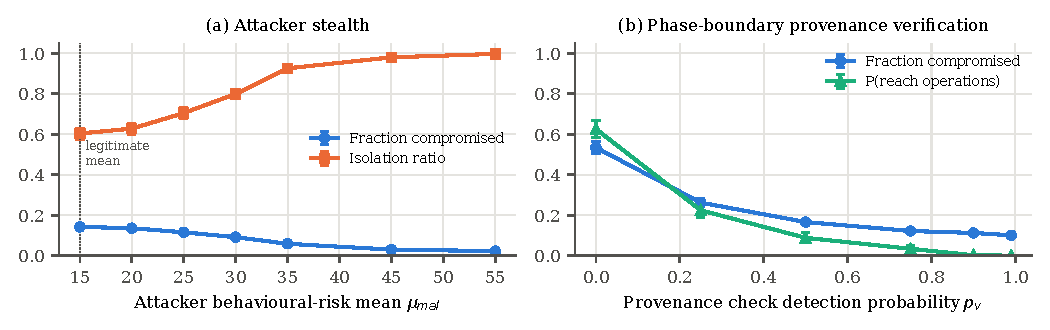
\includegraphics[width=\textwidth]{figs/fig_sensitivity.pdf}
\caption{E1 sensitivity of \ztas{}: (a) effect of attacker stealth $\mu_{\mathrm{mal}}$ on spread and isolation ratio; (b) effect of the provenance-check detection probability $p_v$ on spread and on the probability of reaching operations (stealthy attacker).}
\label{fig:sens}
\end{figure*}

\subsection{Operating Characteristic of the Risk Engine}
Fig.~\ref{fig:roc} shows E2. Mode-dependent weights dominate uniform weights at every operating point. At the step-up threshold $\theta_1=30$, the production-mode weights escalated 69.6\% of noisy and 11.2\% of stealthy malicious requests, against 32.5\% and 1.5\% for uniform weights, while escalating 0.02\% of legitimate requests. The thresholds from the thesis exposed a design problem: with our score distributions \emph{no} single request, legitimate or malicious, exceeded $\theta_2=70$, so the block and isolate tiers were never reached by per-request evidence alone. This finding motivated the evidence-accumulation rule in Section~\ref{sec:arch-risk}: escalation to quarantine must come from repeated failures rather than from one extreme score. In a deployment, thresholds should be calibrated against measured score distributions rather than fixed in advance.

\begin{figure}[!t]
\centering
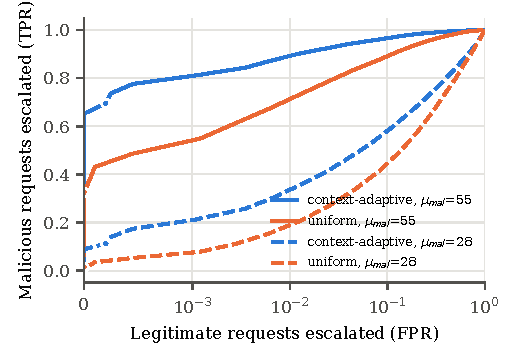
\includegraphics[width=\columnwidth]{figs/fig_roc.pdf}
\caption{E2: fraction of malicious versus legitimate requests escalated beyond \emph{allow} as the threshold varies, for production-mode and uniform weights and two attacker profiles. Markers show $\theta_1=30$. The $x$-axis is linear below $10^{-3}$ and logarithmic above.}
\label{fig:roc}
\end{figure}

\subsection{Cost of Provenance and Post-Quantum Identity}
Table~\ref{tab:sig} lists the measured signature costs. ML-DSA verification (115--195~$\mu$s) is comparable to classical verification (92--102~$\mu$s), but signing with the portable implementation is about 225--310 times slower than Ed25519 (6.5--8.9~ms), and signatures and public keys are one to two orders of magnitude larger. SLH-DSA-128f signatures are 17~kB. ML-KEM-768 encapsulation and decapsulation took 63 and 77~$\mu$s, against 30~$\mu$s for an X25519 exchange, with a 1088-byte ciphertext. One hash-chain step cost 0.48~$\mu$s, and one risk-score evaluation with tiering cost 1.1~$\mu$s (median), so neither is a bottleneck.

\begin{table}[!t]
\centering
\caption{E3: Measured signature costs for a 256-byte provenance record (median of 3000 runs; 100 for SLH-DSA)}
\label{tab:sig}
\footnotesize
\begin{tabular}{@{}lrrrr@{}}
\toprule
Scheme & Sign ($\mu$s) & Verify ($\mu$s) & Sig.\ (B) & PK (B) \\
\midrule
Ed25519 & 28.7 & 102.4 & 64 & 32 \\
ECDSA-P256 & 28.5 & 92.3 & 71 & 64 \\
ML-DSA-44 & 6488.8 & 114.8 & 2420 & 1312 \\
ML-DSA-65 & 8894.8 & 194.5 & 3309 & 1952 \\
SLH-DSA-SHA2-128f & 13191.3 & 855.3 & 17088 & 32 \\
\bottomrule
\end{tabular}
\end{table}

Signing every record individually with ML-DSA-65 would limit a gateway core to about 113 records/s. Merkle batching removes this limit (Fig.~\ref{fig:batch}): the per-record signing cost fell from 8.8~ms at $B=1$ to 140~$\mu$s at $B=64$ and 9.3~$\mu$s at $B=1024$, equivalent to about $1.1\times10^5$ records/s per core. The authenticator overhead per record (amortized signature plus inclusion proof) is lowest at $B=64$ (244~B) and rises slowly beyond it as proofs lengthen. The cost of batching is latency: a record is not signed until its batch closes. For a 1~kHz sensor stream and $B=64$, this adds up to 64~ms, acceptable for provenance and audit but not for closed-loop control. Control commands should therefore be signed individually, or with a classical-plus-PQ hybrid, on the fast path.

\begin{figure*}[!t]
\centering
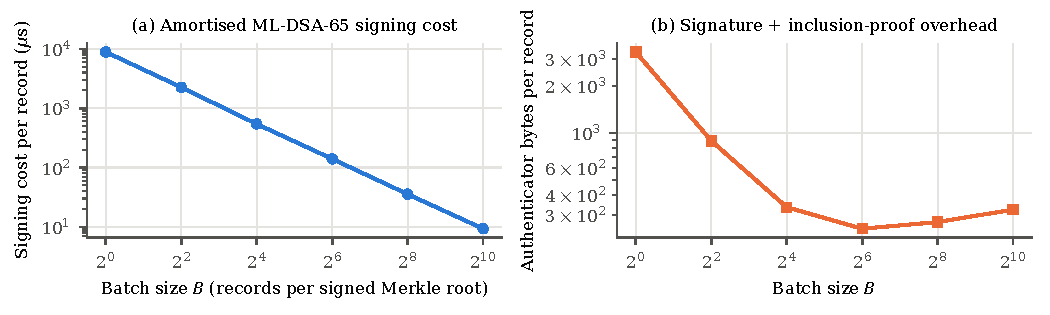
\includegraphics[width=\textwidth]{figs/fig_batching.pdf}
\caption{E3: Merkle batching of provenance records with ML-DSA-65. (a) Measured signing cost per record; (b) bytes of signature and inclusion proof per record.}
\label{fig:batch}
\end{figure*}

% =====================================================================
\section{Discussion}
\label{sec:discussion}
% =====================================================================
\subsection{Interpretation and Practical Implications}
Three observations follow from the results. First, in a lifecycle-spanning system the most valuable control point is the \emph{phase boundary}. Static zones already place a conduit there, but they inspect traffic rather than lineage. Checking signed lineage at the boundary is what stopped propagation in our model, and it worked even against attackers that the behavioral engine could not distinguish from legitimate users. Second, per-request zero-trust authentication is necessary but not sufficient. An adversary that holds a legitimate entity's credentials passes it, so containment depends on mechanisms that look at \emph{what} is being moved and \emph{how} the requester behaves. Third, post-quantum provenance is affordable for DTh records if signing is amortized over batches. It is not yet affordable for per-message control traffic on constrained devices, which argues for a two-path design: batched PQ signatures for lineage and audit, and fast individual (hybrid) signatures for commands.

For practitioners, \ztas{} can be assembled incrementally from existing components; the thesis proposed Keycloak for identity, Open Policy Agent as the decision point, a service mesh such as Istio for flow-scoped segmentation, Hyperledger Fabric for the ledger and an ELK stack for monitoring. The architecture also maps onto existing obligations: provenance and signed change control support the audit requirements of ISO~27001 and sector quality standards, and segments can be expressed as IEC~62443 conduits with time and purpose limits.

\subsection{Threats to Validity}
\emph{Construct validity.} The simulation abstracts each mechanism as a probability ($p_a$, $p_{\mathrm{act}}$, $p_v$, step-up failure) and models risk scores as Gaussian distributions. The absolute numbers therefore depend on these parameters, and the baseline parameters were not tuned to favor or penalize any configuration. We report the parameters, sweep the most influential ones and release the code so that others can substitute their own.

\emph{Internal validity.} The baselines are deliberately simple abstractions of IEC~62443 zoning and SP~800-207 deployments. Real deployments may include additional controls, such as deep-packet inspection of OT protocols, that would narrow the gap.

\emph{External validity.} The graphs are synthetic and of moderate size (60 entities), and real DTh topologies, flow schedules and attacker behavior may differ. The cryptographic measurements were taken on a server-class CPU with a portable PQ implementation. Edge gateways with HSMs and PLC-class microcontrollers will show different absolute costs, and ledger consensus latency was not measured.

\subsection{Limitations}
This work has not been validated on an industrial testbed or in a pilot deployment, and we make no claim of performance in production. The thesis's conclusion chapter mentioned formal model checking and an approximately 60\% attack-surface reduction, but neither was carried out in that work, so we do not report them here. Human factors, regulatory variation and the economics of deployment are outside the scope of this paper.

% =====================================================================
\section{Conclusion and Future Work}
\label{sec:conclusion}
% =====================================================================
The digital thread turns the product lifecycle into a single data path, and with it a single attack path. This paper presented \ztas{}, a zero-trust architecture designed around that path. It treats twins as principals, scores requests with a mode-dependent five-dimensional risk model, scopes segments to data flows and activities, and verifies post-quantum-signed lineage wherever data crosses a lifecycle phase. In a reproducible propagation study, \ztas{} contained a stealthy attacker to about a tenth of the thread and kept it out of the operations phase in more than 99\% of runs, while perimeter, zone-based and static zero-trust baselines allowed 77--99\% of the thread to be compromised. Ablation showed that phase-boundary provenance verification provides most of this effect, and measurements showed that Merkle batching makes ML-DSA signing of provenance records feasible at high record rates.

Future work will (i) implement \ztas{} with open-source components and evaluate it on a hardware-in-the-loop manufacturing testbed, using MITRE ATT\&CK for ICS techniques~\cite{alexander2020attackics} as the attack corpus; (ii) measure latency, throughput and resource overhead on edge gateways and PLC-class devices, including ledger consensus; (iii) calibrate risk weights and thresholds from field data; and (iv) evaluate the approach on real DTh topologies obtained from industrial partners.

\section*{Data and Code Availability}
The simulation code (\texttt{sim\_propagation.py}), benchmark code (\texttt{bench\_crypto.py}), figure scripts and raw results (\texttt{results\_sim.json}, \texttt{results\_crypto.json}) are provided as supplementary material and will be deposited in a public repository upon acceptance.

\bibliographystyle{IEEEtran}
\bibliography{refs}

\end{document}
